\documentclass[a4paper]{article}

%% Language and font encodings
\usepackage[english]{babel}
\usepackage[utf8x]{inputenc}
\usepackage[T1]{fontenc}
\usepackage{xeCJK} 
%% Sets page size and margins
\usepackage[a4paper,top=3cm,bottom=2cm,left=3cm,right=3cm,marginparwidth=1.75cm]{geometry}
\usepackage{fontspec, xunicode, xltxtra}

%% Useful packages
\usepackage{amsmath}
\usepackage{graphicx}
\usepackage[colorinlistoftodos]{todonotes}
\usepackage[colorlinks=true, allcolors=blue]{hyperref}
\usepackage{listings}
\lstset{numbers=left, numberstyle=\tiny,basicstyle=\small, keywordstyle=\color{blue!70}, commentstyle=\color{red!50!green!50!blue!50}, frame=shadowbox, rulesepcolor=\color{red!20!green!20!blue!20},escapeinside=``, xleftmargin=2em,xrightmargin=2em, aboveskip=1em}

\begin{document}
% Titlepage & ToC
\hypersetup{pageanchor=false,
             bookmarksnumbered=true,
             pdfencoding=unicode
            }
\pagenumbering{roman}
\begin{titlepage}
\vspace*{7cm}
\begin{center}%
{\LARGE \textbf{Report of MOOC} }\\
\vskip 1cm

\includegraphics[width=1in]{Logo_ENSIIE.png}
\vskip 1cm
{\Huge \textbf{---------------------------------------------} }\\
\vskip 0.5cm
{\Huge \textbf{Machine Learning} }\\
\vskip 0.5cm
{\Huge \textbf{---------------------------------------------} }\\
\vskip 1cm
\vspace*{1cm}
{\large Guangyue CHEN}\\
\vspace*{0.5cm}
{\large{2018/12/12}}
\end{center}
\end{titlepage}
\tableofcontents{\LARGE}
\pagenumbering{arabic}
\hypersetup{pageanchor=true}


\newpage
\section{\textbf{Methodology}}

\subsection{Linear Model}

For this problem, the linear models have bad performances, but there are also a way to build a linear model. Here we tried `linear regression' , `Ridge Regression' and ` Lasso Regression'. To make some features working such as `DayOfWeek', `StoreType' and `Assortment', we use the ont hot function from package `mltools'. As the results,  all of these three regression have a test error feedbacked from kaggle.com which is arroud 0.4. 

\subsection{\textbf{SVM}}

	For the SVM method, we choose the package ``e1071" to train our model, so our first step is choosing the regression type and the kernel for this regression. 

	\subsubsection{Kernels and Type selection:}

	\begin{center}
	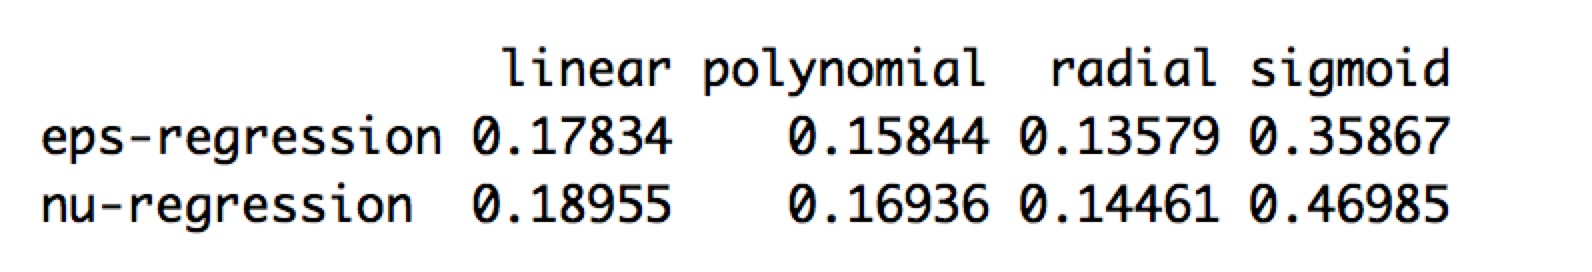
\includegraphics[width=5in]{svmkernal.png}\\
	FigureX: Train Error with different kernels and types used in SVM regression
	\end{center}

	We can see that with the Kernel `radial' and the type `eps-regression', the model permance better.

	\subsubsection{Parameter Choosing:}

	Here we use the function `tune.svm' from the package ``e1071" to compare the different gamma and cost. This function use K-ford cross validation to choose the parameter. The gamma parameter defines how far the influence of a single training example reaches. The cost parameter rules the error of the cutting plane. With higher cost the train error will be lower but the test error may growth, and the parameter gamma is for the Kernel, it's also sensitive for our model.

	\begin{center}
	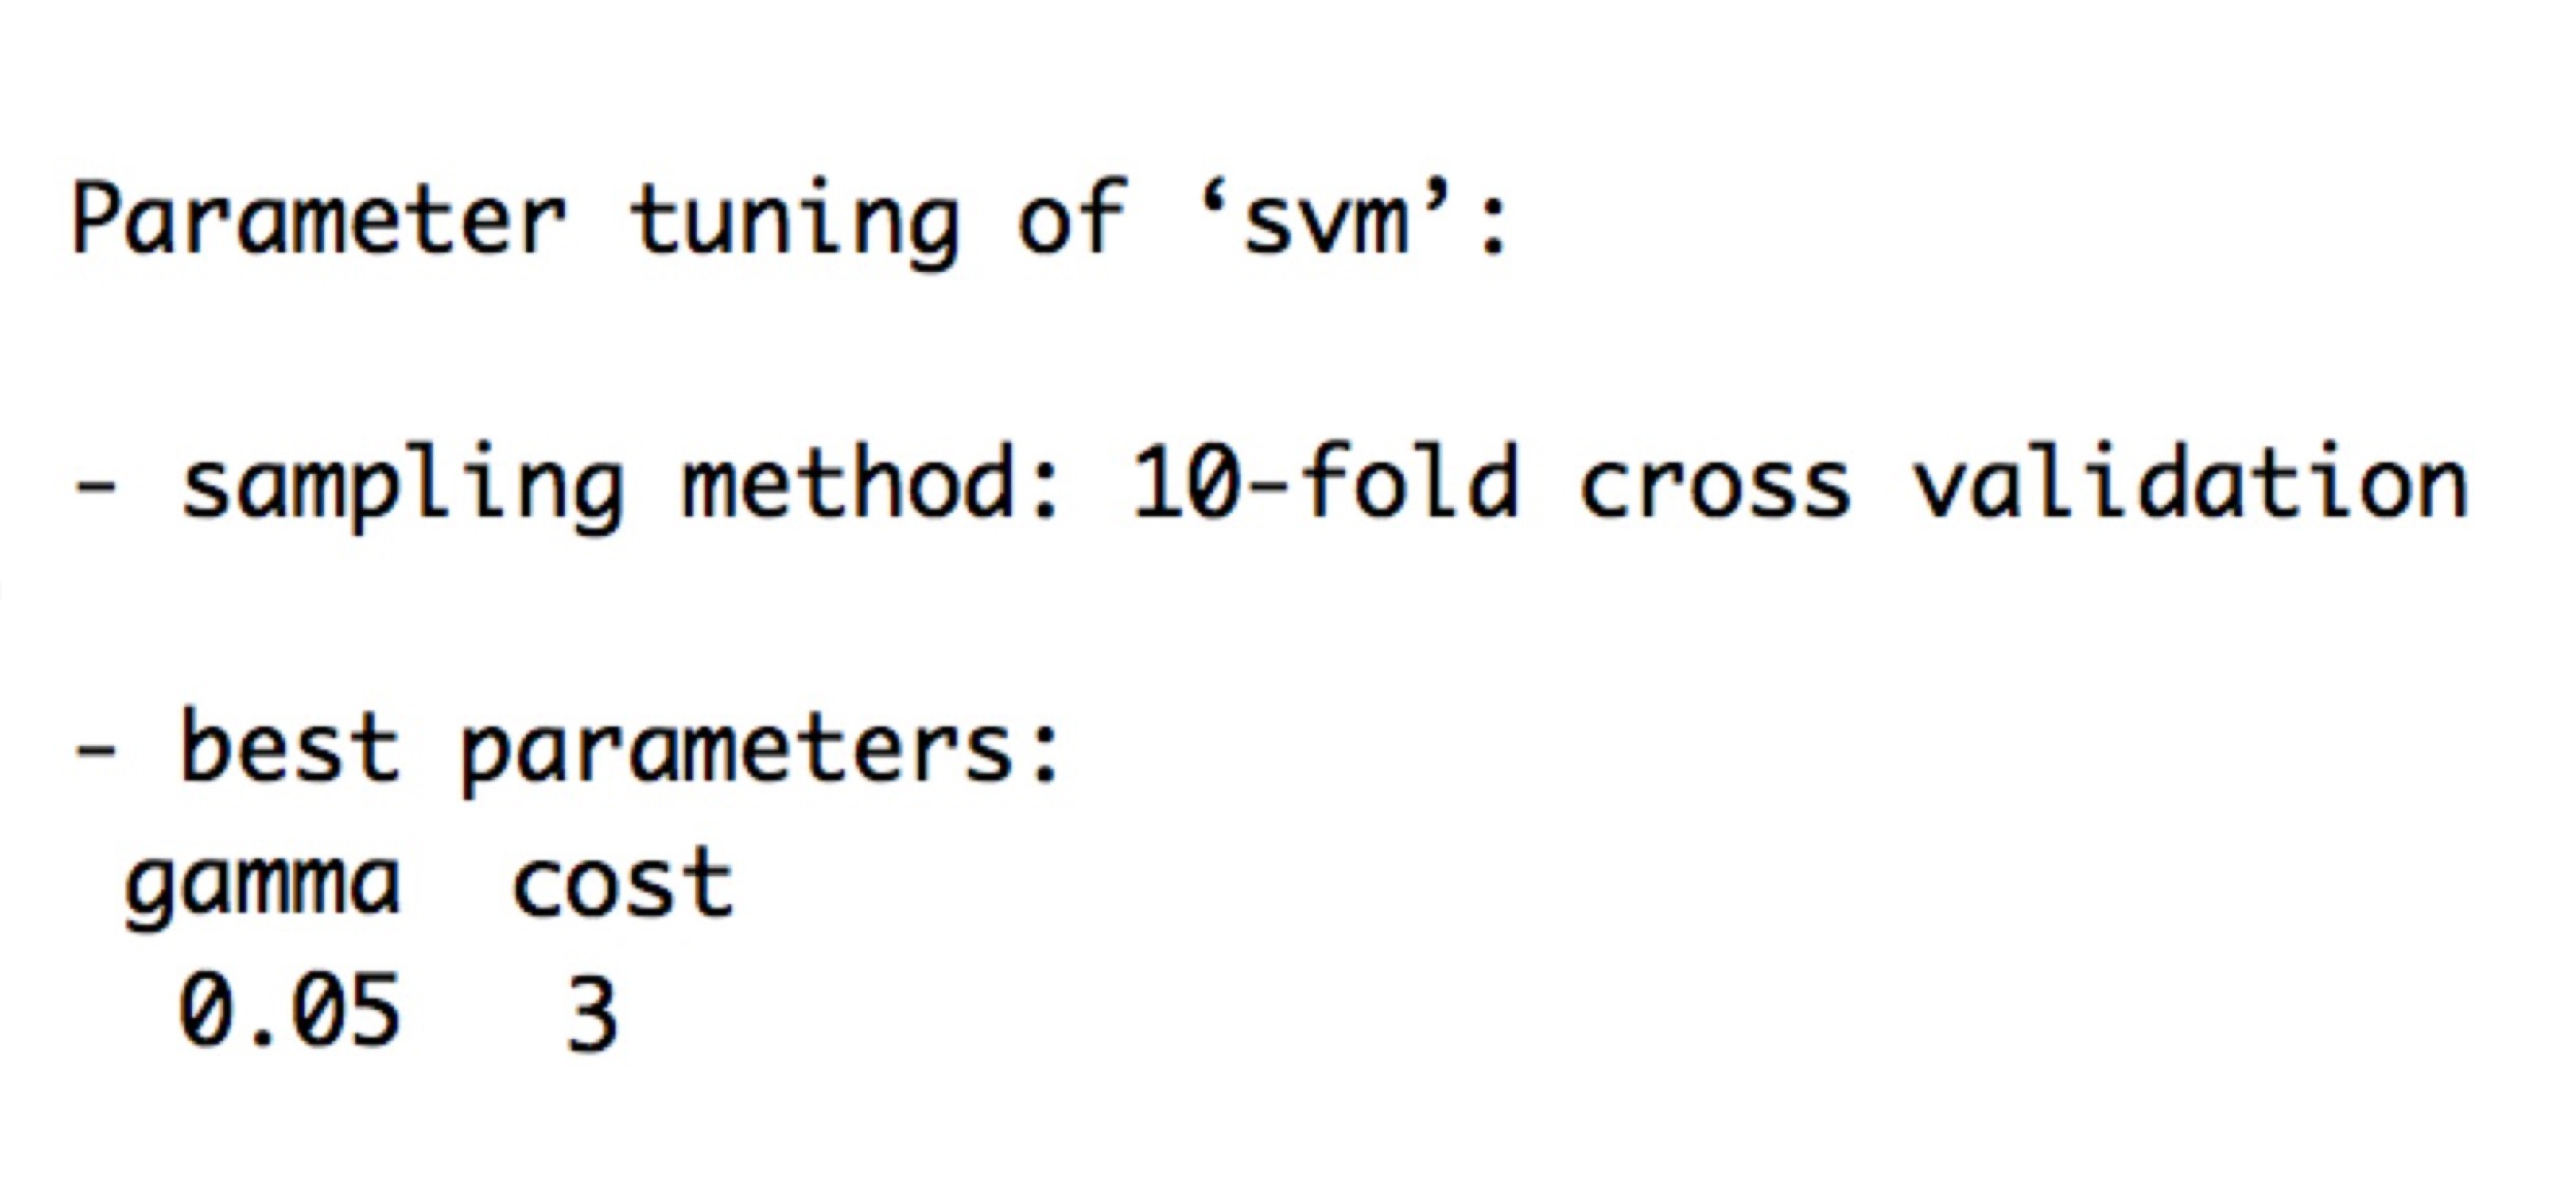
\includegraphics[width=5in]{svmp.jpeg}\\
	FigureX: Best Parameter
	\end{center}

	\subsubsection{Result:}

	Because of the running time of the svm model is long, we didn't pay too much attention into this model. Our result error is .

	\begin{center}
	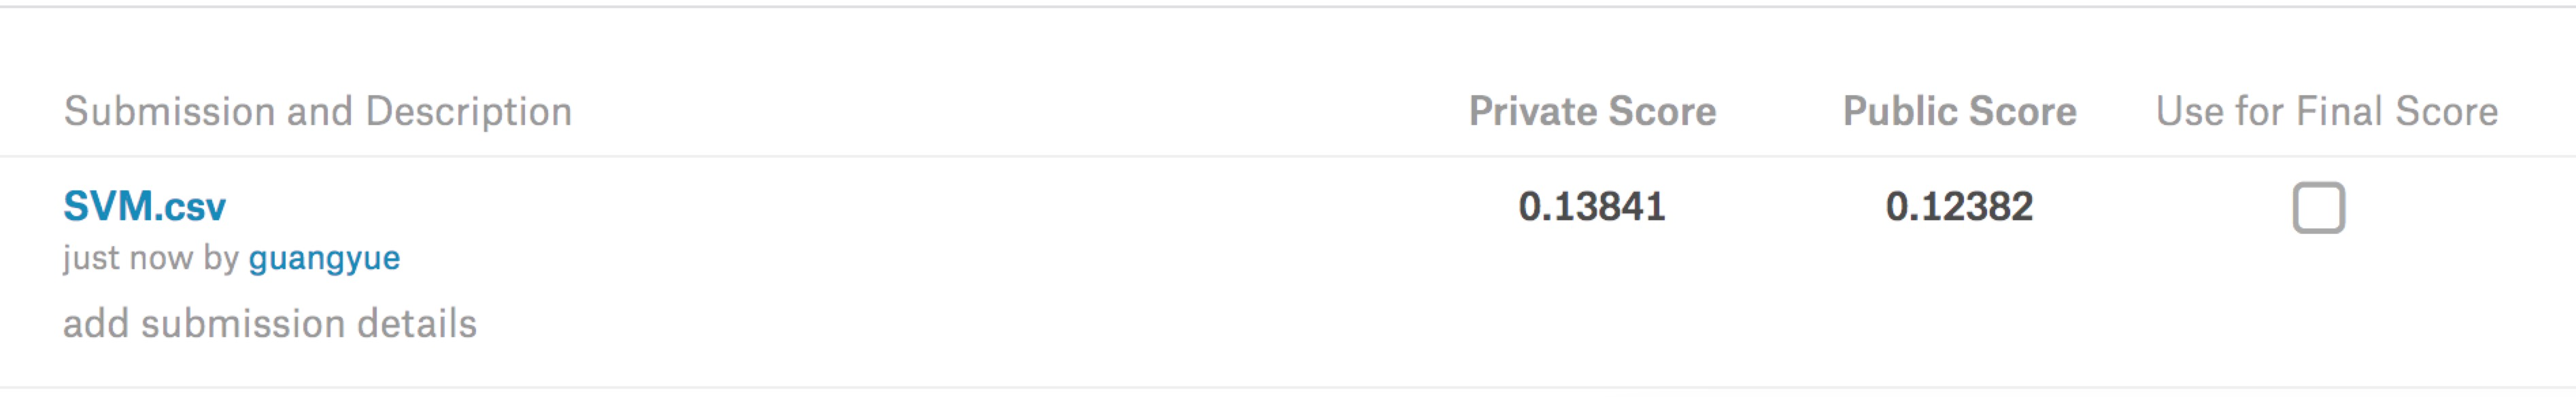
\includegraphics[width=5in]{svmres.png}\\
	FigureX: Result
	\end{center}

\subsection{Random Forest and H2o}

	\subsubsection{Random Forest:}
	
	Random Forest is a flexible, `easy to use' machine learning algorithm, it porduce a good result most of the time. It is also one of the most used algorithms, because it's simplicity and the fact that it can be used for both classification and regression tasks.

	When given a set of data, Random Forest generates a forest of classification or regression trees, rather than a single classification or regression tree. Each of these trees is a weak learner built on a subset of rows and columns. It chose the features and the subset of the data(for training a tree) randomly. More trees will reduce the variance. So it could handle well the overfitting issues. For our problem, it has also a good performance.

	\subsubsection{H2o Random Forest:}

	`H2o' package use Distributed Random Forest, which is a powerful classification and regression tool. For this package, `h2o.randomforest' run faster than the normal one in R, it can also limit the tree depth, (R's randomForest builds really deep trees), allowing for having a better predictions.

	\subsubsection{Parameter Choosing:}

	So here we should choose the parameter `max\_depth', here we use Cross-Validation to compare the test error.

	\begin{center}
	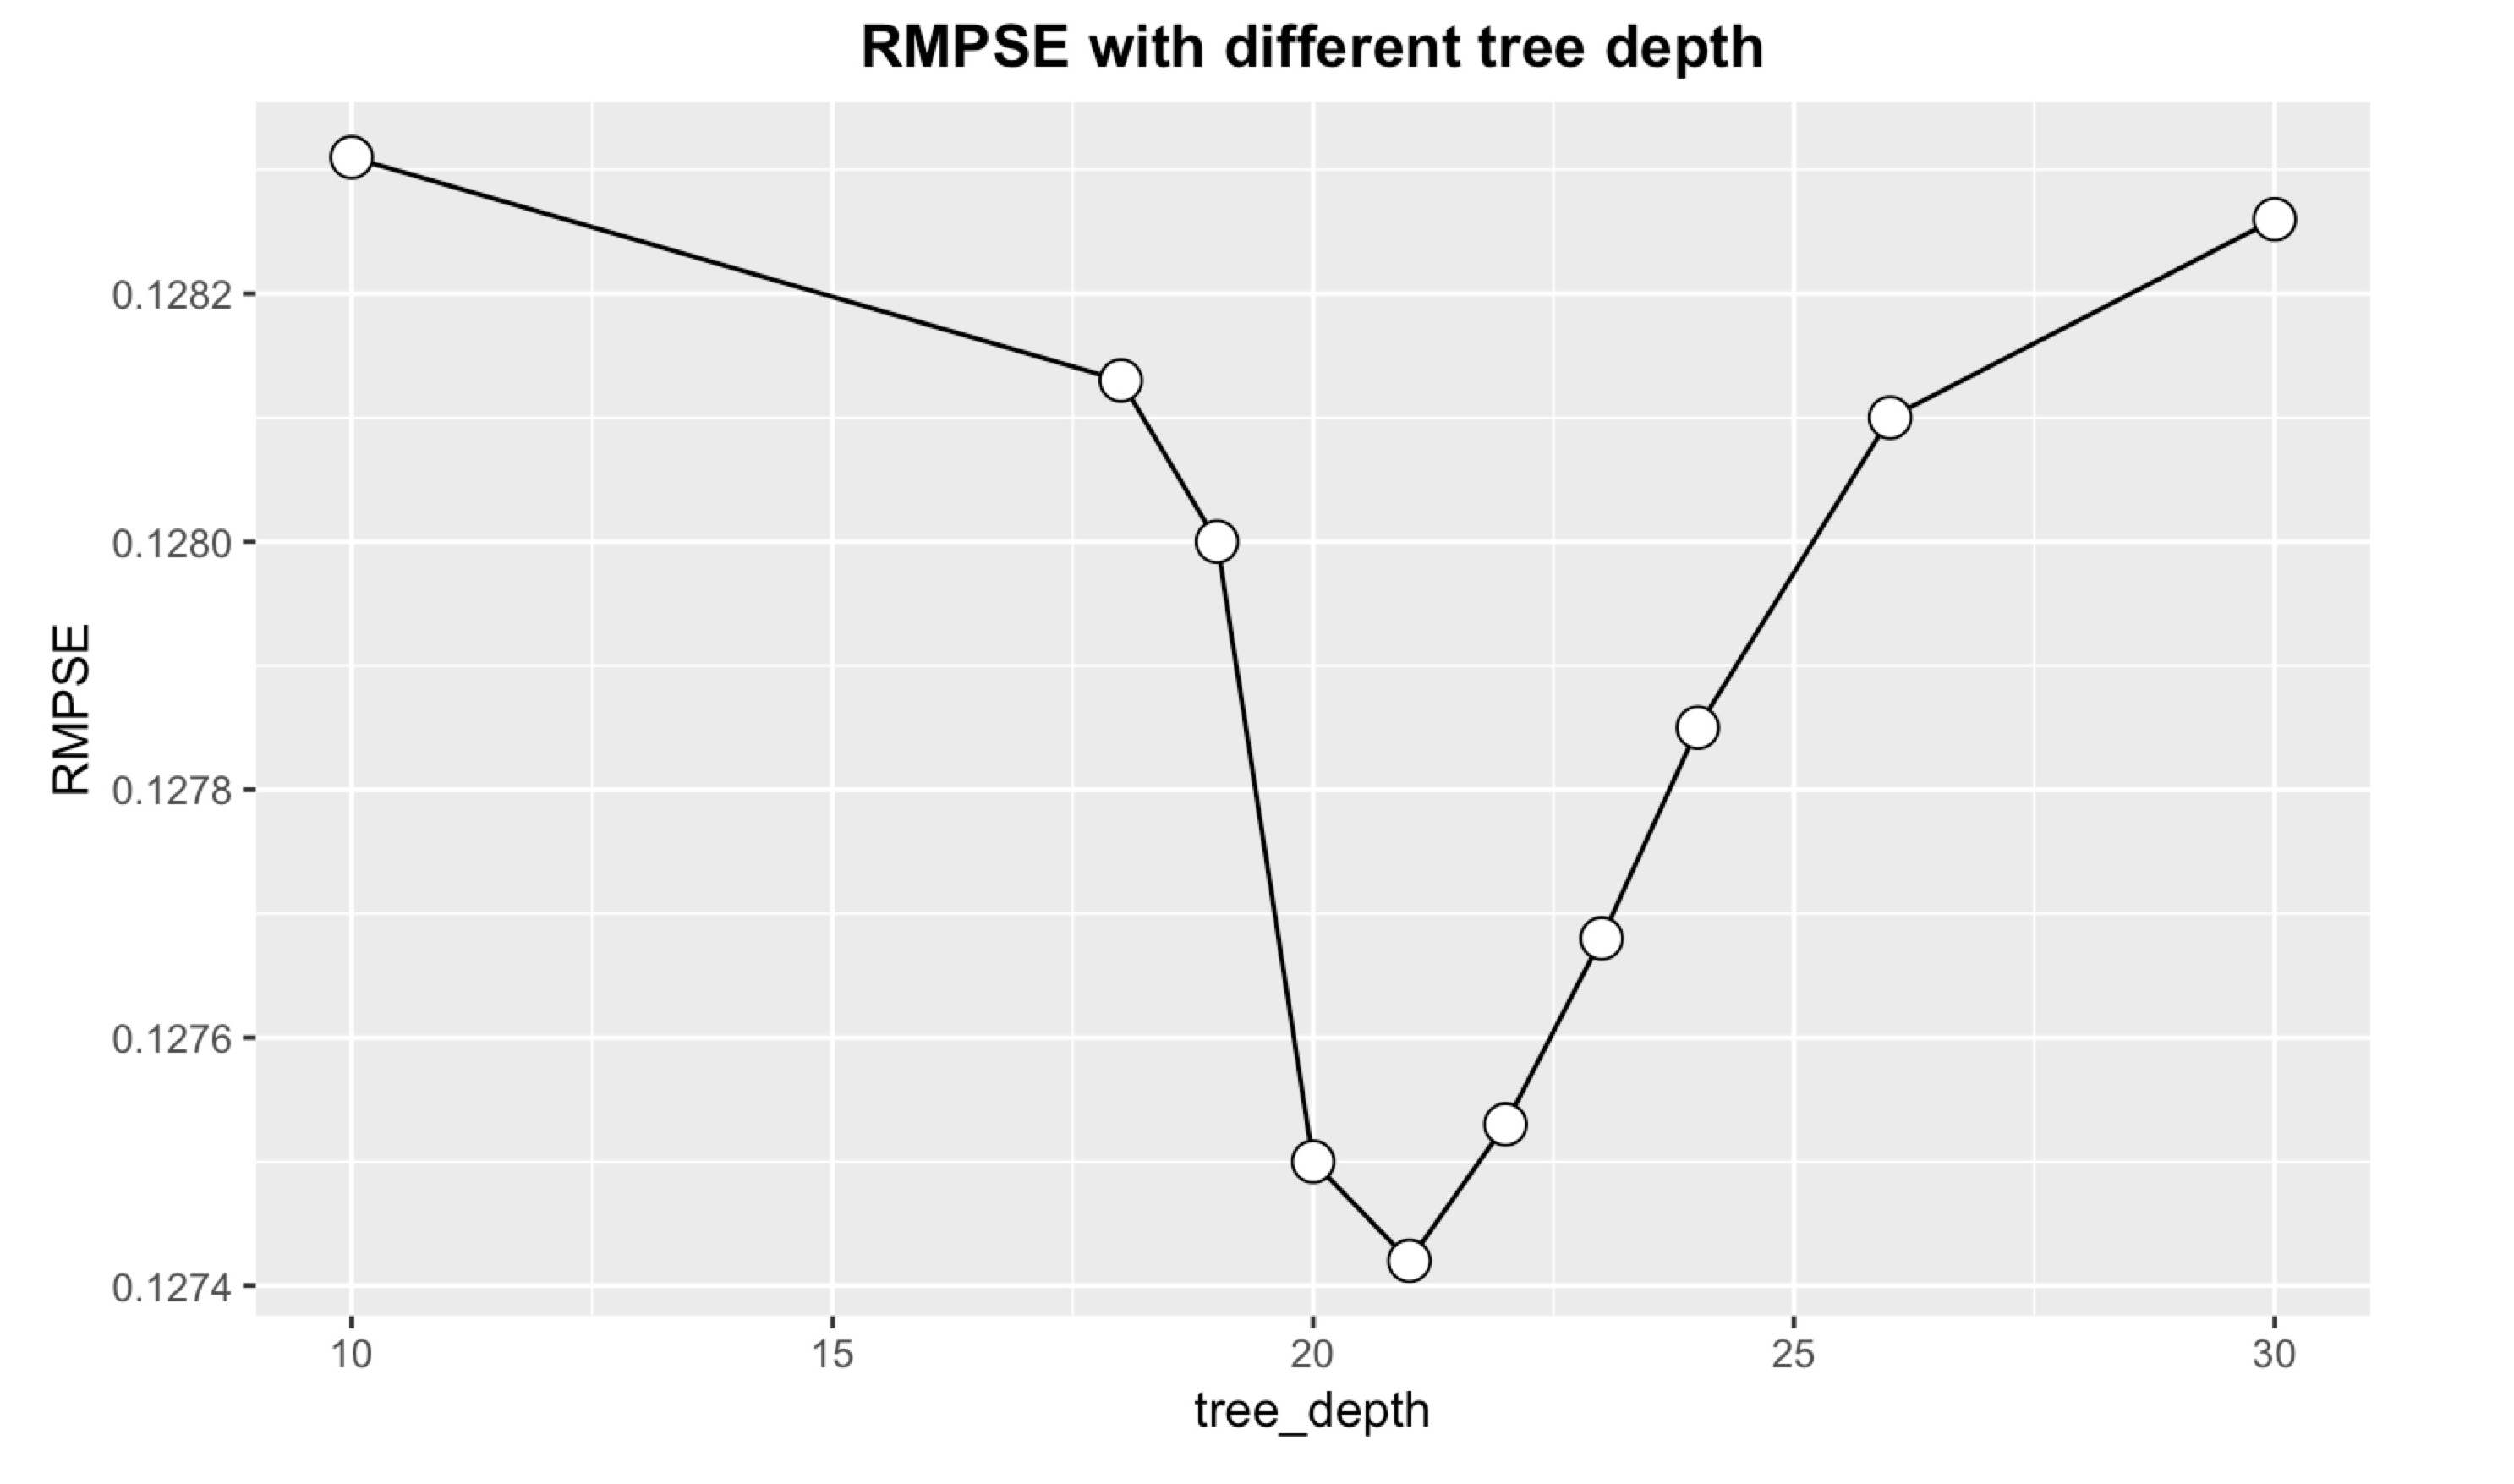
\includegraphics[width=5in]{cross.png}\\
	FigureX: RMPSE with different tree depth
	\end{center}

	We can see that for the test error, the models with depths 20 and 21 have the best porfermences. So we decided to build two models with the depth which are 21 and 20. Then we build a forest with a big quantity of trees, Which is 100.

	\subsubsection{Feature Selection:}

	For h2o random forest, we should load the data into h2o cluster. After our several test, we find that some features make the models perform worse. With the summary of our model, we decide to remove some features which have a low importance to our model. After we remove two features `SchoolHoliday' and `StateHoliday', our random forest model perform better.

	\subsubsection{Result:}

	\begin{center}
	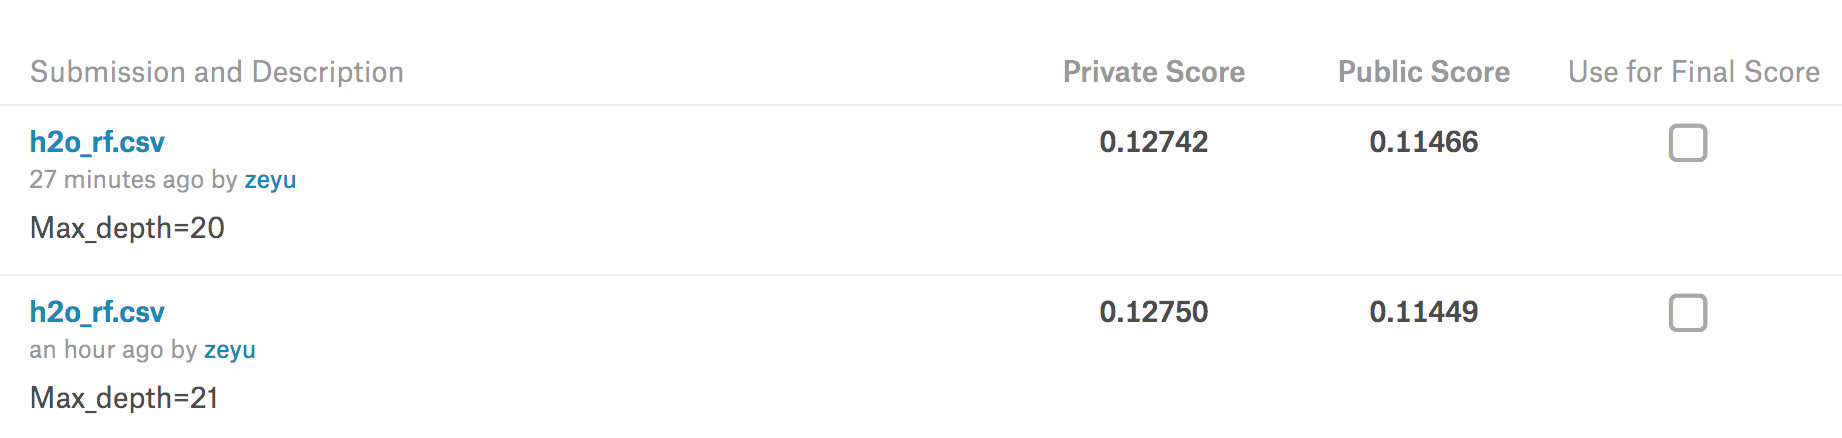
\includegraphics[width=5in]{h2ores.png}\\
	FigureX: The Result Of Our Models
	\end{center}	

	We run our best models on kaggle.com provided test data. The test errors feedbacked	from kaggle.com are 0.11449 and 0.11466. So we can say that the forest with depth maximum 21 is better. And this result is already in the top 150 on kaggle.com. 
\newpage
\section{\textbf{Conclusion}}

According our results,  Random Forest has the lowest test error feedbacked from kaggle.com. But we believe that the SVM model could perform as well as RF although it cost so much time for learning once. So for our future work, we will do more anlyses and tries on SVM.

After this project, we realize that the feature treatment has a large impact on training model quality. A correct feature selection could helps us to develop simpler and faster models. Once features are chosen and formatted correctly, the prediction error improved dramatic. Data preprocessing is the same, because, the representation and quality of data is first and foremost before running an analysis. 

What's more, after this project, we have an unforgetable experience of data analysis. We know clearly the steps to treat the data and train the machine learing models, and have a clearer understanding of models such as Random Forest and Support Vector Machine.

\section{\textbf{Reference}}

1. Data source:\href{https://www.kaggle.com/c/rossmann-store-sales/data}{https://www.kaggle.com/c/rossmann-store-sales/data}

2. Distributed Random Forest Introduction:\href{http://docs.h2o.ai/h2o/latest-stable/h2o-docs/data-science/drf.html}{http://docs.h2o.ai/h2o}

3. Data preprocessing and feature selection:(en chinois)\href{https://blog.csdn.net/u010089444/article/details/70053104}{https://blog.csdn.net}

4. Support Vector Machine: \href{http://uc-r.github.io/svm}{http://uc-r.github.io/svm}

\end{document}